% begin module piecewise-formula
\begin{frame}
\begin{example} %[Example 9, p. 18]
Find a formula for the function $f$ in the graph.

\psset{xunit=1.2cm, yunit=1.2cm}
\begin{pspicture}(-0.5, -0.5)(5.3,2.4) 
\tiny
\psframe*[linecolor=white](-0.5,-0.5)(5.2,2.4) 
\psaxes{<->}(0,0)(-0.5,-0.5)(5.2,2.2)
\psLabels{5.1}{2.2}
\psline[linecolor=red](0,0)(1,1)(2,0)(5,0)
\psHollowDot{5}{0}
\psFullDot{0}{0}
\only<4-5>{
\psline[linecolor=blue](-0.5, -0.5)(2,2)
}
\only<6-7>{
\psline[linecolor=blue](-0.2, 2.2)(2.5,-0.5)
}
\only<8-9>{
\psline[linecolor=blue](2, 0)(5,0)
}
\end{pspicture} 
%\ \only<1-3,10>{%
%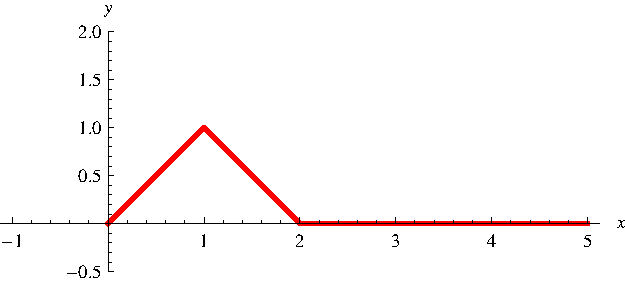
\includegraphics[height=4cm]{precalculus/pictures/01-01-ex-09a.pdf}%
%}%
%\only<handout:0| 4-5>{%
%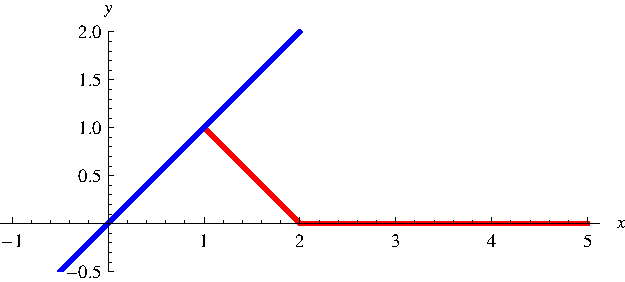
\includegraphics[height=4cm]{precalculus/pictures/01-01-ex-09b.pdf}%
%}%
%\only<handout:0| 6-7>{%
%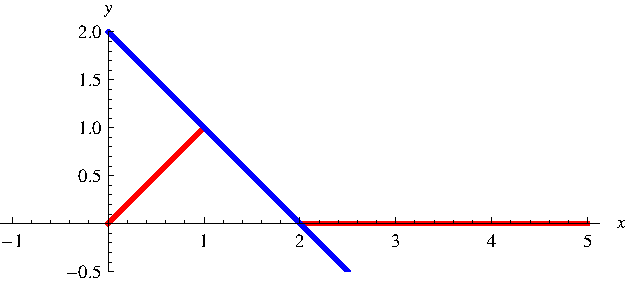
\includegraphics[height=4cm]{precalculus/pictures/01-01-ex-09c.pdf}%
%}%
%\only<handout:0| 8-9>{%
%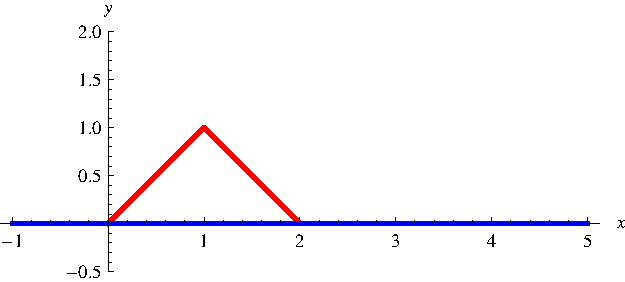
\includegraphics[height=4cm]{precalculus/pictures/01-01-ex-09d.pdf}%
%}%

\uncover<2->{
Different formulas on $[0, 1)$, $[1, 2)$, and $[2, 5)$. 
}

\uncover<3->{
\[
f(x) = \left\{ \begin{array}{ccccccl}
\uncover<5->{\alert<handout:0| 5>{x}} & \alert<handout:0| 4-5>{\textrm{if}} & \alert<handout:0| 4-5>{0} & \alert<handout:0| 4-5>{\leq} & \alert<handout:0| 4-5>{x} & \alert<handout:0| 4-5>{<} & \alert<handout:0| 4-5>{1} \\
\uncover<7->{\alert<handout:0| 7>{2 - x}} & \alert<handout:0| 6-7>{\textrm{if}} & \alert<handout:0| 6-7>{1} & \alert<handout:0| 6-7>{\leq} & \alert<handout:0| 6-7>{x} & \alert<handout:0| 6-7>{<} & \alert<handout:0| 6-7>{2} \\
\uncover<9->{\alert<handout:0| 9>{0}} & \alert<handout:0| 8-9>{\textrm{if}} & \alert<handout:0| 8-9>{2} & \alert<handout:0| 8-9>{\leq} & \alert<handout:0| 8-9>{x} & \alert<handout:0| 8-9>{<} & \alert<handout:0| 8-9>{5} \end{array}\right.
\]
}
\end{example}
\end{frame}
% end module piecewise-formula
